\documentclass{article}

%若使用中文,使用xeLatex编译,并使用XeCJK宏包
\usepackage{xeCJK}

% if you need to pass options to natbib, use, e.g.:
%     \PassOptionsToPackage{numbers, compress}{natbib}
% before loading neurips_2018

\usepackage[final]{neurips_2018}

% to avoid loading the natbib package, add option nonatbib:
%     \usepackage[nonatbib]{neurips_2018}

\usepackage[utf8]{inputenc} % allow utf-8 input
\usepackage[T1]{fontenc}    % use 8-bit T1 fonts
\usepackage{hyperref}       % hyperlinks
\usepackage{url}            % simple URL typesetting
\usepackage{booktabs}       % professional-quality tables
\usepackage{tikz}
\usepackage{amsfonts}       % blackboard math symbols
\usepackage{nicefrac}       % compact symbols for 1/2, etc.
\usepackage{microtype}      % microtypography
\newfontfamily\urlfontfamily{FandolSong-Regular}
\def\UrlFont{\urlfontfamily}

\title{2018-2019学年第二学期COMP130137.01\\
《模式识别与机器学习》课程项目\\
2019语言与智能技术竞赛-机器阅读理解}

\author{\\
学号:17307130155 , 姓名:黄文皓,贡献: 29\%,签名:\\
学号:17307130156 , 姓名:李洪嵚,贡献: 38\%,签名:\\
学号:17307130196 , 姓名:解润芃,贡献: 33\%,签名:\\}

\begin{document}
\begin{center}
  声明:我已知悉学校对于考试纪律的严肃规定,将秉持诚实守信宗旨,严守考试纪律,不作弊,不剽窃;若有违反学校考试纪律的行为,自愿接受学校严肃处理。
\end{center}
\maketitle

\begin{abstract}
   Machine reading comprehension is a basic assignment in natural language processing. There're many useful concept and models that can perfectly understand the text and perform well in Q\&A, such as BiDAF and BERT. However, these models are designed for English text reading, which focus on both characters and words. We fine tune the model so that it can fit the requirement of Chinese text reading. Also we try some other models to answer different form of query. Test result shows that our model achieve almost the same score of the baseline on this Chinese QA task.
\end{abstract}

\section{Overview}
\subsection{Introduction}
Machine Reading Comprehension (MRC) means to let machine read context and then answer the question based on the materials. MRC is an important frontier in the field of natural language processing(NLP) and artificial intelligence(AI). And this is also a hot test to check the ability of a NLP model.The dataset of this competition focus on the problems which are hard to answer in 2018 Machine Reading Comprehension Technology Competition. 

\subsection{Assignment}

The answers to the questions can be divided into three classes: answer the questions through the sentences picked from the materials, answer "yes" or "no", and pick out entity. We mainly focus on the first two kinds of questions in this project. 
As for the first kind of question: the participation reading comprehension system is required to automatically analyze the problem and the candidate document, and output a text answer \emph{a} that satisfies the question based on a given question \emph{q} and its corresponding text form candidate document set \emph{D = d1, d2, ..., dn}. The goal is that \emph{a} can answer the question \emph{q} correctly, completely, and concisely.
And for the "yes or no" questions, the answers will simply be "yes" or "no".

\subsection{About Dataset}
The dataset contains about 280,000 real problem from Baidu Research, and each of them correspond to 5 candidate document and manual answer. The data set is divided into a training set of 270,000 questions, a development set of approximately 3,000 question, and a test set of approximately 7,000 questions.

\section{BERT and BiDAF Introduction}
In this task, we mainly use two models: BERT and BiDAF. The body of the model is BiDAF, and use BERT as the embedding method.
\subsection{BERT}
BERT, which stands for Bidirectional Encoder Representations from Transformers, is a new language representation model. BERT is designed to pre-train deep bidirectional representations from unlabeled text by jointly conditioning on both left and right context in all layers. As a result, the pre-trained BERT model can be finetuned with just one additional output layer to create state-of-the-art models for a wide range of tasks, without substantial task-specific architecture modifications.\citet{DBLP:journals/corr/abs-1810-04805}
\begin{figure}[h]
	\centering
	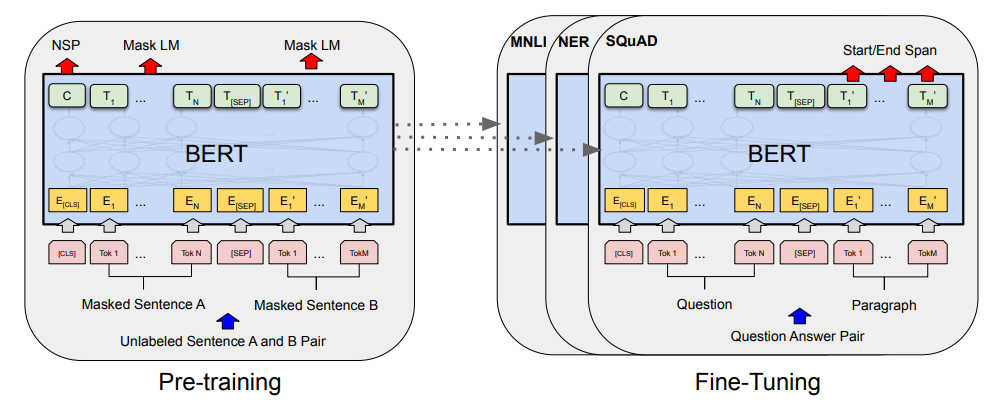
\includegraphics[scale=0.4]{bert.png}
	\caption{Overall pre-training and fine-tuning procedures for BERT}
\end{figure}

\subsection{BiDAF}
Bi-Directional Attention Flow (BiDAF) network is a hierarchical multi-stage architecture for modeling the representations of the context paragraph as different levels of granularity. BIDAF includes character-level, word-level,  \citet{DBLP:journals/corr/SeoKFH16}
\begin{figure}[h]
	\centering
	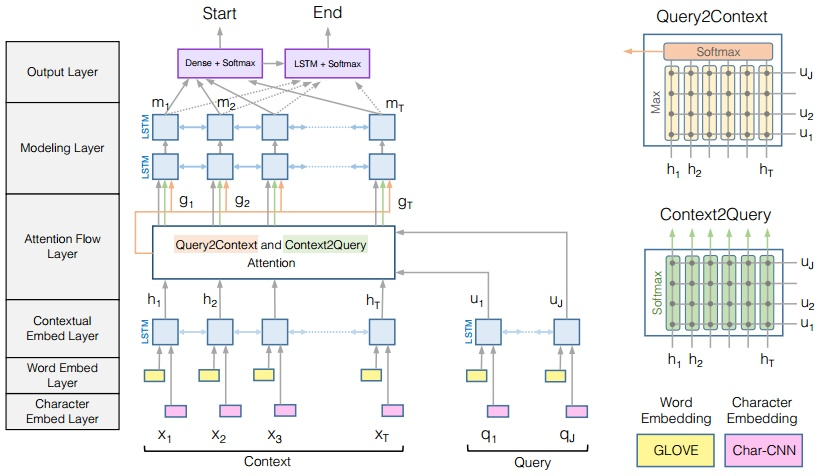
\includegraphics[scale=0.5]{bidaf.jpg}
	\caption{BiDirectional Attention Flow Model}
\end{figure}

\section{Data Preprocessing}
\subsection{Label choice}
The dataset is organized in .json format, which provides various labels about the query and context. After we observe some of them, however, we found that not all the labels is useful. For example, the label "answer" and "fake\_answer" both provide corresponding answer about the query. But the former is generated manually, and the latter is extract from the context. For simplicity, we regard the latter as our target.
\subsection{Text preprocessing}
Considering the dataset contains real problem from Baidu Research, most of the context and query is Chinese. Besides, we found that the context contains lots of incorrelative characters like "20170113", "<span>...</span>", "jkefsgasscd". They don't provide any useful information about how to solve the problem. So we decide to omit all English letter and other non-Chinese character. We gain the text which only has Chinese character and punctuation.In my opinion, it can express the meaning of query and answer better, and it can improve the performance of our model.

Besides, it would take lots of time for BERT to maps query and context to embedding vector when the vocabulary is large. Some words like "是"、"你"、"做" appears frequently, and most of the query and context can be expressded in a simply way. That is, we can use small dictionary to express the paragraph. In this assignment, we set 6000 as the size of the dictionary. It can be proved that BERT can generate corresponding vector in a short time.
\subsection{Data format conversion}
We have to convert data from text to vector that fit the input of the model. Each words in dictionary will embed in a 768-dimension vector. 

\section{Model}
After a simple introduction to the two models, we will dive deeper into the structures of two models in details to see how these models help solving the QA task.
\noindent Our model is a multi-stage process and consists of two parts(Figure 3):\\
\begin{enumerate}
	\item \textbf{BERT} maps each word in query and context to a vector  
	\item \textbf{BiDAF} maps query and context vector in the beginning and ending position of the answer.
\end{enumerate}
\subsection{BERT}
We didn't reproduce the BERT model in this task, but we will make a simple introduction to the model, and see how it works in our task. 
BERT itself is a combination of two important parts: the model and the pre-train methods. 
The model is a mixture of various ideas like attention and transformer. BERT is short for Bidirectional Encoder Representations from Transformers. From one aspect, it's an extension of the idea of word2vector. And in this task, we only use the developed vectors trained by BERT to do the embedding job. 
And the highlights of BERT lie in its pre-train works. The first is the masked language model. It uses random masks to do the prediction work, which makes the model understand the context better. Besides, it uses the nest-sentence prediction to build a connection between the sentences, which enables the model to undertand the sentences better. Therefore, after the two kinds of pre-train, the models will capture both the meaning of characters and sentences. And this is the key point to use vectors produced by BERT.
However, plain BERT is not suitable to solve tasks in Chinese. For one thing, a character usually implies nothing in Chinese, unlike a word in English. The pre-train vectors made by Google uses Chinese characters to do the pre-train work. For higher accuracy, pre-train under words in Chinese is necessary.
\subsection{BiDAF}

Notations: 
lenCon: the length of the context.

lenQue: the length of the query.

$D_H$: the size of the hidden layer.

BiDAF is the main part of this model. BiDAF is short for Bi-directional Attention Flow, which means it uses backward and forward information to achieve this task. In fact, the BiDAF model is a combination of Bi-LSTM and attention, which are both suitable for QA problem.

In this task, we reproduce BiDAF and makes some changes to match QA in Chinese better. Before we dive into BiDAF, we will first have a overview of this model. BiDAF is a model with six layers originally, but we only have four layers indeed. The original six layers are character embeddign layer, word embedding layer, contextual embedding layer, attention flow layer modeling layer and output layer, which in our model, the character embedding layer and word embedding layer are replaced by a pre-trained matrix provided by BERT. 

Word embedding layer and character embedding layer: These two layers transform words and characters into embedding vectors. Since we have used BERT to do the embedding work, the importance of these layers decreases. Therefore, the real inputs are embedded matrixs produced by pretrained BERT. And we don't have enough resources to train BERT or even fine-tune it, we will simply fixed the output of BERT to do the embedding.

Contextual embedding layer: This layer is simply a BiLSTM which makes the model have a general view of the whole passage. Since BiLSTM is wildly used in many models, we will not introduce the structure of the model in details. BiLSTM makes each word in the sentences have the opportunity to contacts the context, which is useful for a better comprehension of this character, since we don not use words to do embedding.

Attention flow layer: This layer is the most important layer in this model. The basic idea of this layer is to get two vectors: c2q and q2c, which makes the model be aware of the connections between the context and query. This layer is also the attention layer as mentioned in the name of BiDAF. This layer trys to make the context to be aware of the query and also to make the query be aware of the context. The computations in this layer is quite complicated. 

To begin with, we have to mention the similarity matrix S(lenCon*lenQue). S[i][j] means the similarity between the i-th character in context and j-th character in query. And $S[i][j]=W[C[i];Q[j];C[i]*Q[j]]+b$.

After we have got the similarity matrix, we need to compute the q2c and c2q matrix. We do the computation in the following way:

$$a_t=softmax(S_{t:})\\U_{:t}=\sum_{j}a_{tj}U_{:j}$$ 
 
To be explicit, this matrix computes the sum of the similarity of each word in the context and the query. And finally, we get a new matrix of $( 2*D_H , lenCon )$. In this way, we get the representations of the c2q. 
As for q2c, the idea is quite the same as c2q. The only difference is the direction to use this matrix. $$b=softmax(max(S))\\h=\sum_tb_tH_{:t}$$. And we get another matrix: $(s*D_H* lenCon)$. One difference here is that the length of context is much longer than the length of the query, so we need the most connnected word between context and query. That's where the max function comes from.

Modeling layer: Like Contextual layer, this layer is a combination of two BiLSTM. It servers for the comprehension of the information fetched from the formor layers. In other words, the layer serves as reconsiderations and conclusions. 

Output layer: Work for this layer is simple: using the data to make predictions of the starts and ends of the answers. As for "yes or no" problem, a simple softmax function will be enough. 

\begin{figure}[h]
	\centering
	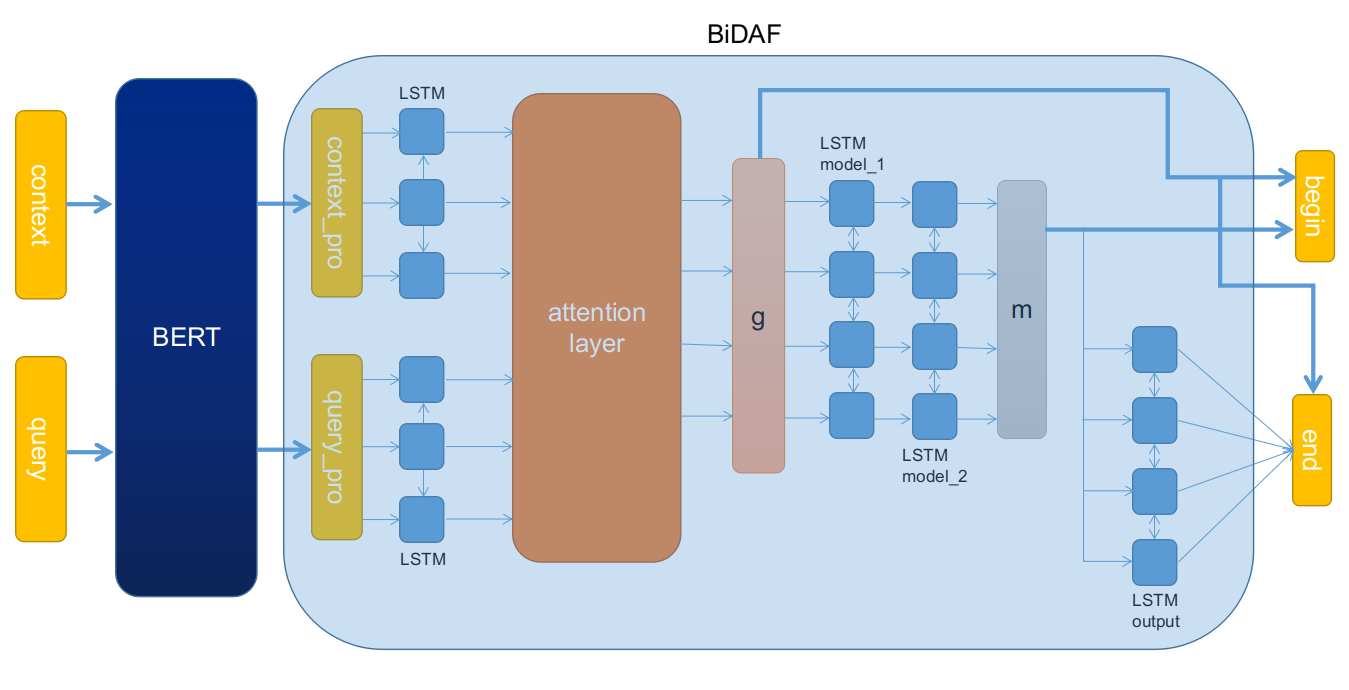
\includegraphics[scale=0.25 ]{Model.png}
	\caption{Model combined by BERT and BiDAF}
\end{figure}

\section{Train}
In our work, we choose a batch size of 10, since the embedding vector is 768 dim and the document length is about 1000~2000 in average. Thus the model cannot fit well into the GPU if larger batch size is applied.

The input of model $X$ is of shape (batch\_size, seq\_len, embedding\_size), e.g. $X[i][j]$ is a vector of j-th word of i-th document 

And the output of the model are spans information with begin index $\hat{bi}$ and end index $\hat {ei}$, both of which are of shape (batch\_size, seq\_len), e.g. $\hat {bi}[i][j]$ is the probability that begin index of i-th document occurs at j-th word of the i-th document.

\begin{figure}[h]
	\centering
	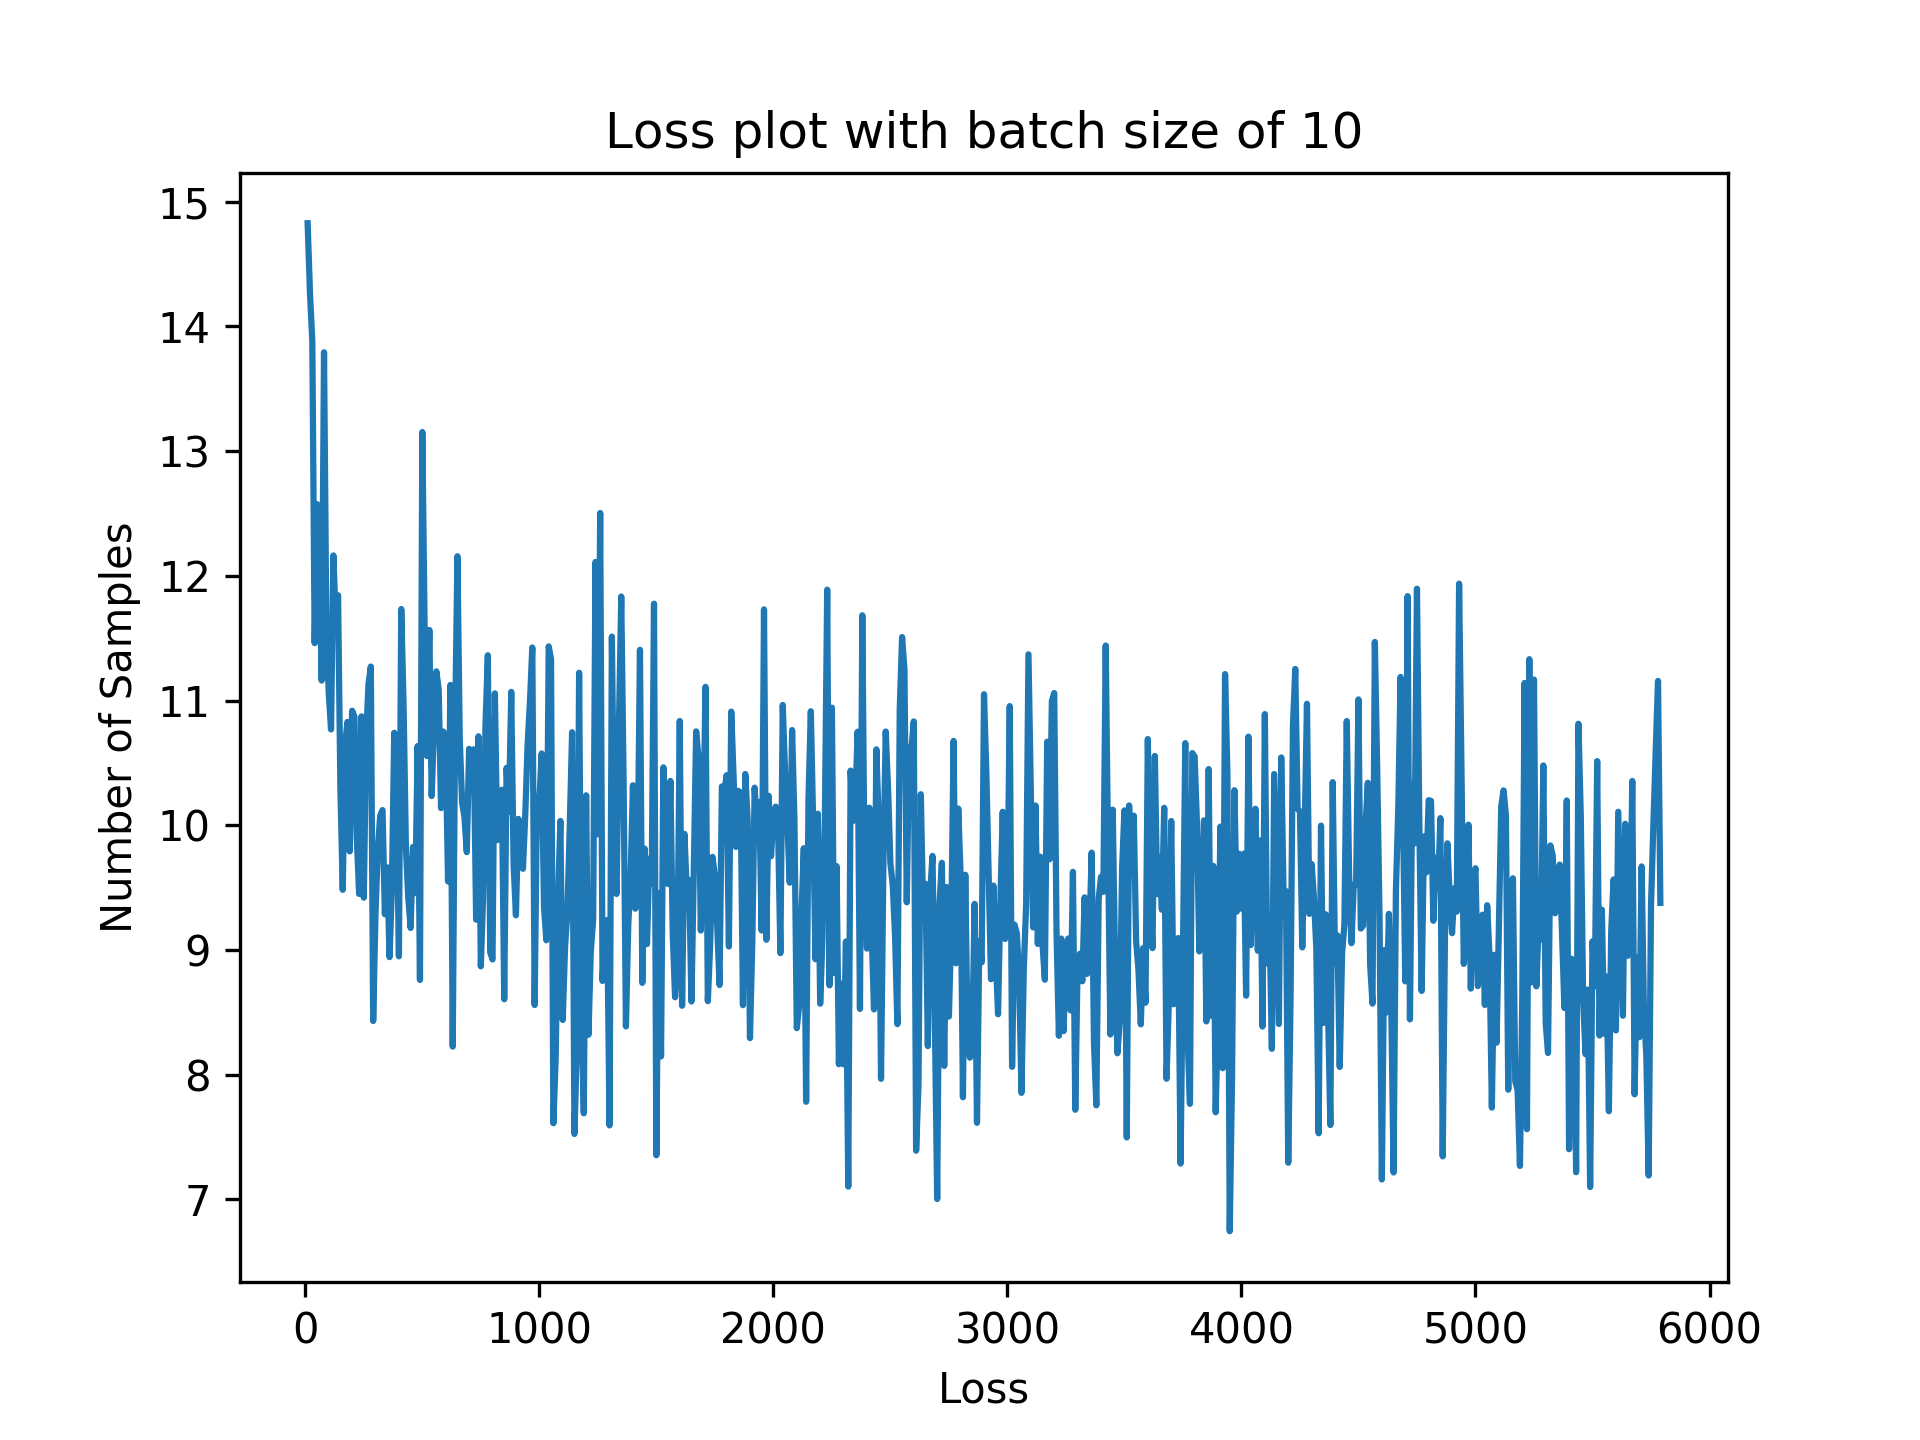
\includegraphics[scale=0.4]{loss.png}
	\caption{Loss curve on training set}
\end{figure}

As for the loss function, since both begin index and end index can be regarded as a classification problem of $seq\_len$ classes, we simply add up the cross entropy of both, i.e. $Loss= CrossEntropy(bi, \hat {bi}) + CrossEntropy(ei, \hat{ei})$, where $bi$, $ei$ are the target begin index and end index respectively and $\hat{bi}$, $\hat{ei}$ are the prediction of begin index and end index given by our model.

\section{Result}
After training on the Baidu Search dataset for only \textbf{one} epoch, we generate the prediction on development set of Baidu Search and use the official scoring script to evaluation our result. The comparison with official BiDAF baseline is shown below. (Notice that the result given by below don't include the bonus for answering yes-or-no or entity, since we haven't implement this part. And that's why the scores below are much more less than those on the leader board. )

BiDAF Baseline provided by Baidu.\citet{DBLP:journals/corr/abs-1711-05073}

Result with question-type-specific model, i.e., we train a model by only yes-or-no questions and another model by other questions, then the prediction of yes-or-no questions are given by the yes-or-no model and other questions are given by another model. (Because the answers for yes-or-no questions are always very short, which is quite different from description and entity questions)

\begin{table}
	\caption{Results on test set}
	\label{result-table}
	\centering
	\begin{tabular}{lll}
		\toprule
		  Model   &  BLEU    & Rough-L \\
		\midrule
		Baidu BiDAF Baseline & 23.1 & 31.1     \\
		Single Model     & 22.56 & 32.53      \\
		Question-type-specific Model     & 20.35 & 33.04  \\
		\bottomrule
	\end{tabular}
\end{table}

As we can see above, our model is able to achieve almost the same score of the baseline on this Chinese QA task. However, a quite strange thing is that although we only use char-level embedding and haven't included the word-level embedding, we can achieve almost the same score of baseline, which utilize both char and word level embedding. We think the possible reasons includes:
\begin{enumerate}
	\item Chinese (in fact, ancient Chinese) character is exactly a word and maybe char-level embedding is quite suitable for Chinese NLP task
	\item The high performance of pretrained vectors given by BERT.
	\item Our preprocessing, only allowing 6000 Chinese character and punctuations, greatly removes the noise of the documents.
\end{enumerate}

\bibliographystyle{plainnat}
\bibliography{references}


\end{document}
